%===================== DESENVOLVIMENTO DO SISTEMA =====================
\section{Desenvolvimento do sistema}

\subsection{Identidade do projeto}

O sistema foi nomeado LibrasAI — Reconhecimento Inteligente de Libras em Tempo
Real. A identidade visual adotada segue uma paleta de cores com significado
semântico direto: azul escuro (\texttt{\#1F3864}), representando a solidez da
tecnologia de IA; azul médio (\texttt{\#2E75B6}), representando a comunicação
fluida entre surdos e ouvintes; e verde (\texttt{\#1E5631}), representando o
impacto social positivo de cada gesto reconhecido com sucesso. A ausência de
elementos decorativos na interface reforça o caráter técnico e científico do
projeto.

\subsection{Pilha tecnológica}

A Tabela~\ref{tab:pilha} apresenta as tecnologias utilizadas e a função de cada
uma no sistema.

\begin{table}[htbp]
\centering
\caption{Pilha tecnológica do LibrasAI.}
\label{tab:pilha}
\small
\begin{tabular}{@{}p{3cm} p{3.6cm} p{6cm}@{}}
\toprule
\textbf{Categoria} & \textbf{Tecnologia} & \textbf{Função} \\
\midrule
Linguagem & Python 3.10+ & Linguagem principal de todo o sistema \\
Aprendizado profundo & TensorFlow 2.13 / Keras & Construção, treinamento e inferência do modelo CNN + LSTM \\
Visão computacional & MediaPipe 0.10.9 & Detecção de mãos e extração de 21 \textit{landmarks} $(x, y, z)$ em tempo real \\
Captura de vídeo & OpenCV 4.8+ & Captura da webcam, processamento de \textit{frames} e renderização da interface \\
Dados & NumPy 1.24+ & Manipulação de \textit{arrays}, normalização e \textit{data augmentation} \\
Avaliação & Scikit-learn 1.3+ & Métricas: F1, Kappa de Cohen, top-k e matriz de confusão \\
Gráficos & Matplotlib / Seaborn & Curvas de treinamento, matriz de confusão e relatório visual \\
Hardware & Webcam USB ou integrada & Único \textit{hardware} necessário; testado a 640$\times$480, 30 FPS \\
\bottomrule
\end{tabular}
\end{table}

\subsection{Estrutura do repositório}

O código-fonte está organizado nos seguintes módulos:

\begin{itemize}[leftmargin=2cm]
  \item \texttt{main.py} — ponto de entrada da aplicação;
  \item \texttt{collect\_data.py} — coleta interativa de amostras;
  \item \texttt{train\_model.py} — treinamento do modelo;
  \item \texttt{predict\_realtime.py} — inferência em tempo real;
  \item \texttt{evaluate\_model.py} — avaliação e geração das métricas;
  \item diretórios \texttt{utils/}, \texttt{dataset/}, \texttt{models/} e
  \texttt{logs/}.
\end{itemize}

\subsection{Interface de reconhecimento em tempo real}

A interface de reconhecimento (\texttt{predict\_realtime.py}) exibe, sobre o vídeo
da webcam, os \textit{landmarks} detectados, o gesto reconhecido com seu
percentual de confiança, as três classes mais prováveis em barras de
probabilidade, o progresso de preenchimento do \textit{buffer} de 50
\textit{frames} e a frase formada até o momento (Figuras~\ref{fig:interface}
e~\ref{fig:frase}).

\begin{figure}[htbp]
\centering
\figpendente{Print da tela principal: \textit{landmarks} sobre a mão, gesto
detectado, barras de confiança (top-3) e barra de progresso do \textit{buffer}.}
\caption{Interface do LibrasAI durante o reconhecimento de um gesto.}
\label{fig:interface}
\end{figure}

\begin{figure}[htbp]
\centering
\figpendente{Print mostrando a frase acumulada na tela e o modo de operação ativo
(WORDS, LETTERS ou MIXED).}
\caption{Formação de frase a partir de gestos reconhecidos em sequência.}
\label{fig:frase}
\end{figure}

\subsection{Plataforma web LibrARs}

Além do protótipo descrito nas seções anteriores, o projeto foi disponibilizado
como uma plataforma web, o LibrARs, acessível pelo navegador do computador ou do
celular, sem instalação de aplicativo. A plataforma serve a dois propósitos: a
coleta colaborativa de dados para a pesquisa e o uso do reconhecimento por
qualquer participante.

% [PENDENTE: definir a relação entre o protótipo em Python (CNN + LSTM) e a
% plataforma web, que hoje usa um classificador por vizinhos mais próximos
% (Seção 5.5.4). Ajustar a Seção 4.4, que descreve o sistema como totalmente
% local.]

\subsubsection{Arquitetura}

A interface é uma aplicação de página única que executa o MediaPipe Hands no
próprio navegador. Apenas os \textit{landmarks} normalizados são enviados ao
servidor; nenhuma imagem ou vídeo sai do dispositivo do participante. O
\textit{backend} expõe uma API REST com três grupos de rotas: autenticação
(cadastro por convite, \textit{login} e redefinição de senha), gestos (cadastro,
listagem e base coletiva) e administração (participantes, estatísticas,
\textit{analytics}, convites e exportação do \textit{dataset}). A chamada em
tempo real usa WebRTC para o vídeo e Socket.IO para a sinalização.

\subsubsection{Fluxo do participante}

O acesso é feito por convite: o administrador gera um \textit{link} válido por 7
dias e o participante cria a conta, informando dados demográficos (sexo, faixa
etária, grau de surdez e conhecimento em Libras). Após o \textit{login}, o painel
do participante (Figura~\ref{fig:painel}) resume os gestos treinados e dá acesso
às funções de tradução, treino e biblioteca.

\begin{figure}[htbp]
\centering
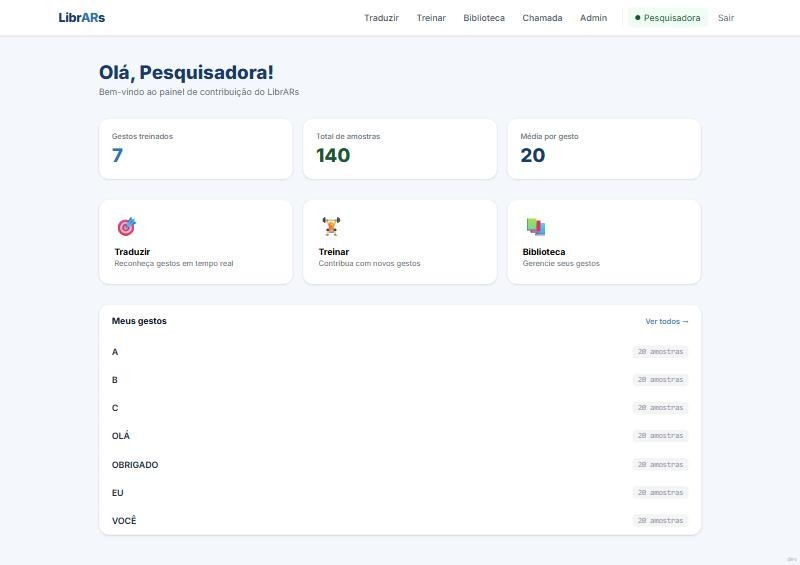
\includegraphics[width=0.85\textwidth]{fig_painel}
\caption{Painel do participante na plataforma LibrARs.}
\label{fig:painel}
\end{figure}

Na tela Treinar, o participante escolhe uma letra do alfabeto ou um sinal comum,
ou digita o nome de um novo gesto, e grava o gesto em frente à câmera. A
plataforma avalia a qualidade da gravação conforme a proporção de quadros em que
a mão foi detectada e orienta o participante a regravar quando a mão sai do quadro
com frequência. Cada gravação armazena até 150 quadros brutos, 20 quadros
amostrados para o classificador estático e um vetor temporal que resume o
movimento.

\begin{figure}[htbp]
\centering
\figpendente{Print da tela Treinar com a câmera ativa: mão detectada, gesto
selecionado e progresso da gravação. (A câmera não pôde ser acessada na captura
automática.)}
\caption{Tela Treinar durante a gravação de um gesto.}
\label{fig:treinar}
\end{figure}

A Biblioteca (Figura~\ref{fig:biblioteca}) lista os gestos do participante e
permite importá-los, exportá-los e carregar a base coletiva, formada pelos gestos
de todos os participantes, para ampliar o vocabulário reconhecido na tradução.

\begin{figure}[htbp]
\centering
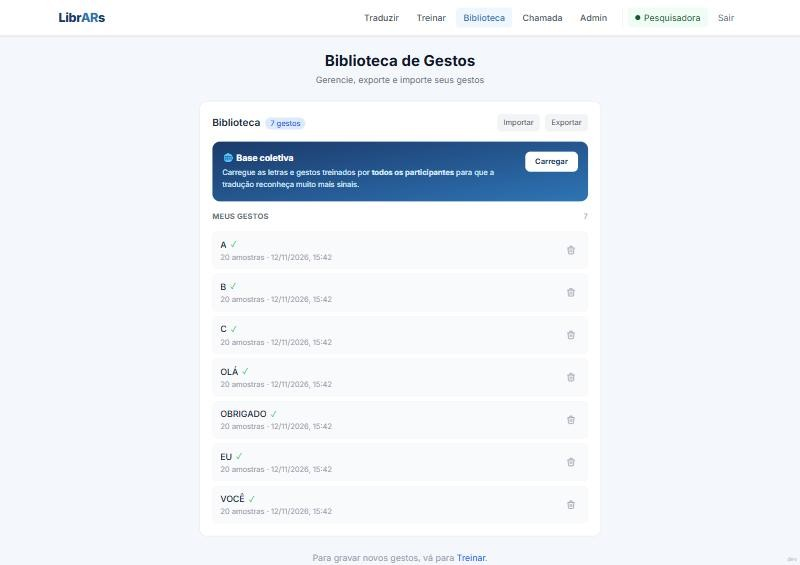
\includegraphics[width=0.85\textwidth]{fig_biblioteca}
\caption{Biblioteca de gestos, com acesso à base coletiva.}
\label{fig:biblioteca}
\end{figure}

A tela Traduzir exibe o gesto reconhecido sobre o vídeo, com uma barra de
confiança (verde a partir de 70\%, amarela entre 45\% e 70\%, vermelha abaixo de
45\%), e acumula os gestos reconhecidos em uma frase. A Chamada
(Figura~\ref{fig:chamada}) permite criar uma sala ou entrar com um código para
uma conversa por vídeo com tradução nos dois sentidos: gestos convertidos em
texto e fala convertida em texto por reconhecimento de voz do navegador.

\begin{figure}[htbp]
\centering
\figpendente{Print da tela Traduzir com a câmera ativa: gesto reconhecido, barra
de confiança e frase detectada.}
\caption{Tela Traduzir reconhecendo um gesto e formando uma frase.}
\label{fig:traduzir}
\end{figure}

\begin{figure}[htbp]
\centering
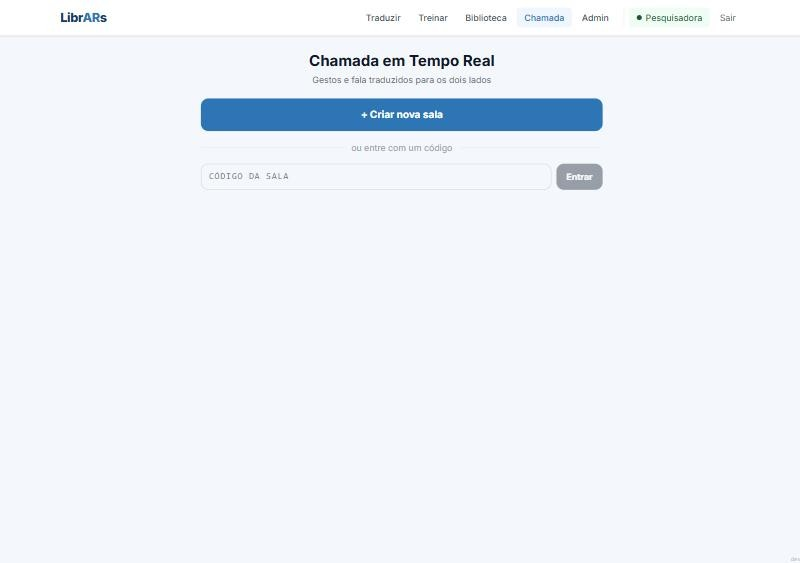
\includegraphics[width=0.85\textwidth]{fig_chamada}
\caption{Tela inicial da chamada em tempo real.}
\label{fig:chamada}
\end{figure}

\subsubsection{Painel do administrador}

O painel do administrador reúne a gestão de participantes
(Figura~\ref{fig:admin-users}), a listagem de todas as gravações
(Figura~\ref{fig:admin-rec}), indicadores de contribuição, a geração de convites
e a exportação do \textit{dataset} bruto em JSON, com os quadros de cada gravação
associados a um identificador do participante. Nas figuras, nomes e e-mails foram
substituídos por identificadores anônimos.

\begin{figure}[htbp]
\centering
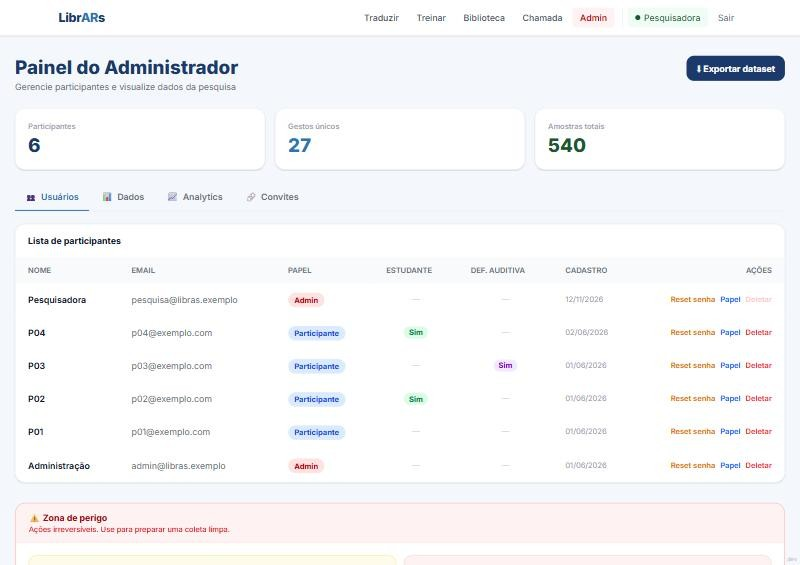
\includegraphics[width=0.9\textwidth]{fig_admin_participantes}
\caption{Painel do administrador: lista de participantes (dados anonimizados).}
\label{fig:admin-users}
\end{figure}

\begin{figure}[htbp]
\centering
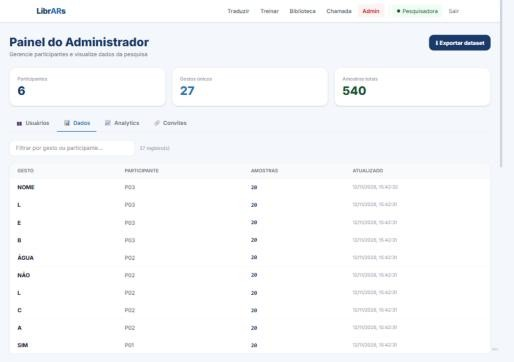
\includegraphics[width=0.75\textwidth]{fig_admin_gravacoes}
\caption{Painel do administrador: gravações por gesto e participante (dados
anonimizados).}
\label{fig:admin-rec}
\end{figure}

\subsubsection{Classificador da plataforma}
\label{subsec:classificador-plataforma}

O reconhecimento na plataforma web não usa a rede CNN + LSTM, e sim um
classificador por $k$ vizinhos mais próximos ($k$-NN) executado no navegador.
Cada quadro é representado pelos 63 valores dos \textit{landmarks}, normalizados
pelo pulso e pela distância pulso–base do dedo médio, como na
Seção~\ref{subsec:pipeline}. A distância entre dois quadros é euclidiana, com peso
0,25 para a coordenada $z$, menos confiável na estimativa monocular. Os 5
vizinhos mais próximos votam com peso inversamente proporcional ao quadrado da
distância, e a predição só é aceita se: (i) o vizinho mais próximo estiver a uma
distância máxima de 1,2; (ii) a confiança do vencedor for de pelo menos 60\%; e
(iii) a diferença para o segundo colocado for de pelo menos 15 pontos percentuais.
Caso contrário, o quadro é rejeitado. Para gestos com movimento, há um caminho
temporal análogo, que compara vetores com média, desvio-padrão, velocidade média
e deslocamento total de cada coordenada ao longo da gravação.
